\documentclass[t, aspectratio=169, english, table]{_style/tudelft-beamer}
% \includeonlyframes{current}% beamer documentation \S 4.3.3

\title[Self-replicating seedboxes]{Self-replicating seedbox servers using programmable money}
\subtitle{EternalSeedBox}
\author{Matei Dogariu}
\date[25 June 2026]{Public thesis defense --- 25 June 2026}
% define a graphic to be shown next to the title
\titlegraphic{
\includegraphics[width=0.4\paperwidth]{icons/design proces/iterations.pdf}}

% optional:
% \setlength{\titlesplitpos}{-0.5\paperwidth}
% mind that in this case, the white pane is the background, and the blue one on top.

\institute{Supervisor: Johan Pouwelse\\Delft University of Technology --- EEMCS}

\addbibresource{bibfile.bib}

\newcommand{\absimage}[4][0.5,0.5]{%
  \begin{textblock}{#3}%width
    [#1]% alignment anchor within image (centered by default)
    (#2)% position on the page (origin is top left)
    \includegraphics[width=#3\paperwidth]{#4}%
\end{textblock}}


\begin{document}


\titleframe

% EDIT intro.tex
{
  \renewcommand{\sectionsubtitle}{Content distribution without a human operator}
  \section{Research Angle}
}


\begin{frame}{Centralized distribution means a single point of control}
  Mainstream content distribution concentrates control on one entity
  that owns both the hardware and the content.
  \begin{itemize}
    \item An operator decides what stays online. Availability depends
      on profitability, policies, and legality.
    \item Peer-to-peer protocols distribute the content
      across many nodes, but the hardware is
      still \emph{managed} by humans.
  \end{itemize}

  \begin{alertblock}{The open research gap}
    Can the \textbf{infrastructure layer itself} be operator-independent, with no human controlling it after genesis?
  \end{alertblock}
\end{frame}

%TODO: add here slide that very briefly details the high level goal of the system, how it fits in the open research gap and how it fixes the two drawbacks mentioned on the slide above. only then it leads into the research question below. 

{
  \setlength{\splitpos}{0.55\paperwidth} % colored pane left, title shifts right
  \leftfooterwhitetrue
  \begin{frame}{Research question}
    \begin{columns}[T]
      \begin{textcolumn}
        \color{white}\large
        Can a network of autonomous software agents, controlled only by inherited economic
        parameters, \textbf{survive} and \textbf{grow} without further human
        intervention?
      \end{textcolumn}
      \begin{textcolumn}
        The hypothesis under test: two outcomes must hold, network
        \textcolor{tud Orange}{persistence} and \textcolor{tud Orange}{expansion},
        with automated control and no human in the loop after genesis.
        
        Falsifiable: survival and growth, can be disproved by data.
      \end{textcolumn}
    \end{columns}
  \end{frame}
}
\setlength{\splitpos}{0pt}\leftfooterwhitefalse % reset stateful split/footer


{
\setbeamerfont{itemize/enumerate body}{size=\small} % template pins lists to \normalsize
\setbeamerfont{footnote}{size=\scriptsize} % shrink full-reference citation footnotes
\footerinfootnotestrue % full-reference footnotes -> move footer into footnote band
\begin{frame}{Where this sits scientifically}
  \small
  \begin{columns}[T, onlytextwidth]
    \begin{column}{0.48\textwidth}
      Prior self-replicators ran on simulated resources:
      \begin{itemize}
        \item von Neumann's automata\cite{vonneumann} and Ray's
          Tierra\cite{tierra}. Running on simulated CPU cycles
          and RAM.
        \item DAOs and autonomic computing self-manage, but only over
          virtual, quota-based resources.
      \end{itemize}

      \textcolor{tud Orange}{\textbf{Research Novelty:}} first self-replicating system on
      \textbf{real infrastructure paid for with real money}.
    \end{column}
    \begin{column}{0.48\textwidth}
      We propose three contributions:
      \begin{enumerate}
        \item \textbf{Engineering} --- first self-replicating economic agent that
          buys real infrastructure on an open market.
        \item \textbf{Method} --- unmodified production code run against a replica
          Bitcoin network and a mock VPS marketplace.
        \item \textbf{Empirical} --- fleet dynamics and one heritable trait under
          selection.
      \end{enumerate}
    \end{column}
  \end{columns}
\end{frame}
}


{
  \renewcommand{\sectionsubtitle}{How a node lives, reproduces, mutates, and dies}
  \section{The system}
}


{
\setbeamerfont{itemize/enumerate body}{size=\small} % template pins lists to \normalsize
\begin{frame}{System at a glance: one autonomous node}
  \small
  \begin{columns}[T, onlytextwidth]
    \begin{column}{0.46\textwidth}
      A node is one process running on a leased SporeStack (a Bitcoin-native marketplace) VPS with:
      \begin{itemize}
        \item \textbf{Bitcoin wallet} --- pays its own bills.
        \item \textbf{Seedbox} --- serves Creative Commons content.
        \item \textbf{IPv8 overlay} --- gossips health telemetry to peers.
        \item \textbf{Decision logic} --- the core actions.
      \end{itemize}

      \textcolor{tud Orange}{No central authority:} bootstraping genesis is the only human action. afterwards the fleet self-governs and no node has authority.
    \end{column}
    \begin{column}{0.5\textwidth}
      \centering
      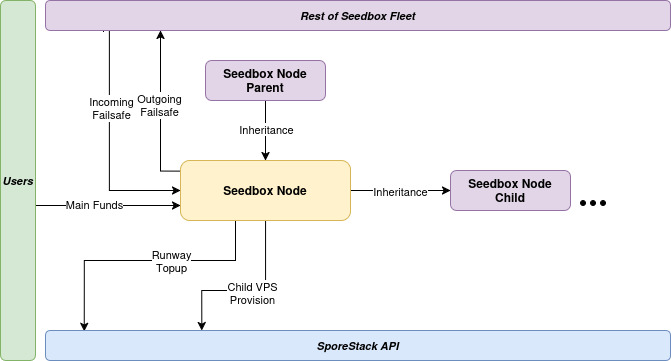
\includegraphics[width=\linewidth]{figures/NodeArchitectureSeedBox.jpg}\\[0.5ex]
      {\footnotesize Arrows trace Bitcoin movements.}
    \end{column}
  \end{columns}
\end{frame}
}


{
\setbeamerfont{itemize/enumerate body}{size=\small} % template pins lists to \normalsize
\begin{frame}{The decision loop}
  \framesubtitle{The main control logic}
  \small
  \begin{columns}[T, onlytextwidth]
    \begin{column}{0.5\textwidth}
      \centering
      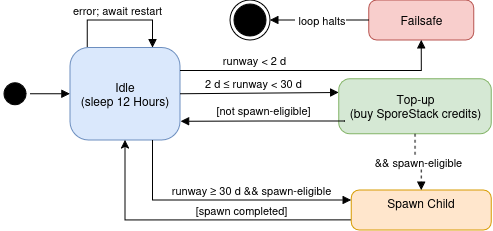
\includegraphics[width=\linewidth]{figures/decision_loop_statemachine.png}
    \end{column}
    \begin{column}{0.46\textwidth}
      Every 12 h, the node takes the first action whose guard passes:
      \begin{enumerate}
        \item \textbf{Failsafe} --- runway \textcolor{tud Orange}{< 2 days}
          \(\to\) sweep remaining funds to the richest peer.
        \item \textbf{Top-up} --- runway < 30 days \(\to\) buy VPS credits to cover another 30 days (\emph{does not end tick}).
        \item \textbf{Spawn} --- if eligible \(\to\) provision + fund a child.
        \item \textbf{Idle} --- wait for the next tick.
      \end{enumerate}

      \medskip
      \textbf{Identical code} runs in every node.
    \end{column}
  \end{columns}
\end{frame}
}


{
\setbeamerfont{itemize/enumerate body}{size=\small} % template pins lists to \normalsize
\begin{frame}{Reproduction mechanics}
  \small
  \begin{block}{Check post-spawn runway, not before}
    A node spawns only if its \textbf{post-spawn total runway}
    \(\geq 60\times(1+\text{caution})\) days \emph{and} its wallet can pay for the
    child's VPS. A node's \textbf{total runway} \(=\) VPS days \(+\) SporeStack credit
    \(+\) BTC.
  \end{block}

  \begin{itemize}
    \item The child starts with a \textbf{30-day} pre-paid VPS and inherits
      \textbf{40\%} of the Bitcoin remaining \emph{after} the parent covers the
      child's expenses.
    \item Actual Pipeline: mutate caution \(\to\) provision VPS \(\to\) fresh BTC wallet \(\to\) deploy code over SSH \(\to\) transfer inheritance.
  \end{itemize}
\end{frame}
}


{
  \setlength{\splitpos}{0.55\paperwidth} % colored pane left, title shifts right
  \leftfooterwhitetrue
  \begin{frame}{The heritable trait}
    \begin{columns}[T]
      \begin{textcolumn}
        \color{white}\large
        \textbf{Caution} --- the single trait under selection.

        \medskip
        \medskip
        \medskip
        \medskip
        \medskip
        \medskip
        Value \(c \in [0.35, 0.9]\), with the genesis node starting at \(c = 0.5\).
        Everything else is inherited.
      \end{textcolumn}
      \begin{textcolumn}
        \footnotesize
        It scales the spawn threshold \(60\times(1+c)\):

        \smallskip
        \begin{tabular}{cc}
          caution \(c\) & threshold \\
          0.35 & 81 days \\
          0.5  & 90 days \\
          0.9  & 114 days \\
        \end{tabular}

        \smallskip
        Low caution \(=\) spawn sooner \\  
        High caution \(=\) retain more 

        \smallskip
        Mutation Formula:\\
        \(c = c_{\text{parent}} + \mathcal{N}(0,0.05)
        + 0.2\,(0.5 - c_{\text{parent}})\) Gaussian drift with reversion to 0.5.

      \end{textcolumn}
    \end{columns}
  \end{frame}
}
\setlength{\splitpos}{0pt}\leftfooterwhitefalse % reset stateful split/footer

%
% Segment 3 --- The method (slides 9--10). Makes the internal-validity
% argument: the lab runs the unmodified production code (only the network
% layer is swapped), and the two experiments differ by one income knob ---
% with the honesty caveat that income sits ~10x above realistic rate.
%

{
  \renewcommand{\sectionsubtitle}{What runs in the lab is the code that would run live}
  \section{The method}
}


{
\setbeamerfont{itemize/enumerate body}{size=\small} % template pins lists to \normalsize
\begin{frame}{Faithful exercise of production code}
  \framesubtitle{Internal validity}
  \small
  \begin{columns}[T, onlytextwidth]
    \begin{column}{0.44\textwidth}
      \begin{block}{Unchanged from live deployment}
        Entrypoint, orchestrator, Bitcoin wallet, and IPv8 community run
        \textbf{identically} to a real deployment --- the only edits concern
        compressed-time intervals: 1 sim-day \(\approx\) \qty{22}{s}, a 90-sim-day
        runway \(\approx\) \qty{32}{min}.
      \end{block}
    \end{column}
    \begin{column}{0.52\textwidth}
      \textbf{Swapped --- network layer only:}
      \begin{itemize}
        \item Bitcoin \(\to\) private \textbf{regtest} (1\,s blocks), same Python
          library paths.
        \item SporeStack API \(\to\) host-side \textbf{mock}, identical endpoints;
          invoices paid in real regtest BTC, mined locally.
        \item Each ``server'' \(=\) a real \textbf{Alpine LXC container} (own FS /
          PID tree / IP); parent deploys over the production SSH pipeline.
        \item Peer discovery via the same IPv8 tracker; a bootstrap container boots
          first, keeping the fleet off the public Internet.
      \end{itemize}
    \end{column}
  \end{columns}

  \textcolor{tud Orange}{\textbf{What runs in the lab is the code that would run live.}}
\end{frame}
}


{
\setbeamerfont{itemize/enumerate body}{size=\small} % template pins lists to \normalsize
\begin{frame}{Two experiments, one income knob}
  \framesubtitle{Closed system vs. open system}
  \small
  \begin{columns}[T, onlytextwidth]
    \begin{column}{0.48\textwidth}
      \textbf{No-income run} --- closed system
      \begin{itemize}
        \item Genesis seeded with one \textbf{€10,000} lump sum; no exogenous
          income.
        \item Every node spends only its birth runway \(+\) inheritance.
        \item A \textcolor{tud Orange}{falsifiable closed-system prediction}: the
          fleet cannot sustain itself indefinitely.
        \item \texttt{faucet\_enabled = false}
      \end{itemize}
    \end{column}
    \begin{column}{0.48\textwidth}
      \textbf{Income run} --- open system
      \begin{itemize}
        \item Host-side income pays the fleet; per-node income \(\approx\)
          invariant (payout scales with node count).
        \item Uneven daily shares (Dirichlet draw).
        \item \textbf{Node cap 60}: income suspended at 60 nodes, resumed below 40
          \(\to\) alternating growth/drought.
        \item \texttt{faucet\_enabled = true}
      \end{itemize}
    \end{column}
  \end{columns}

  \vspace{-1ex}
  \begin{alertblock}{Honesty up front}
    Under load the regtest network drops \(\sim\)half of all broadcasts, so income
    is set at \textbf{\(\sim\)10\(\times\) per-node rent} --- well above any realistic
    seeding rate. \textbf{The income run tests fleet mechanics under favorable
    conditions, not economic viability.}
  \end{alertblock}
\end{frame}
}

% Layout note: the footer (TUD logo + date) is an absolute textpos overlay at
% the page bottom, NOT reserved body space --- so beamer never warns about it,
% but content reaching the bottom ~0.1\paperheight collides with the logo.
% Keep subtitles short (the frametitle template pulls a top image up into a
% long subtitle) and leave the bottom element clear of the footer band.
%

{
  \renewcommand{\sectionsubtitle}{Mechanics confirmed, hypothesis tested}
  \section{Results}
}


{
\setbeamerfont{itemize/enumerate body}{size=\small} % template pins lists to \normalsize
\begin{frame}{No-income run}
\smallskip
\smallskip
\smallskip
  \framesubtitle{Fixed budget predictably spent?}
  \centerline{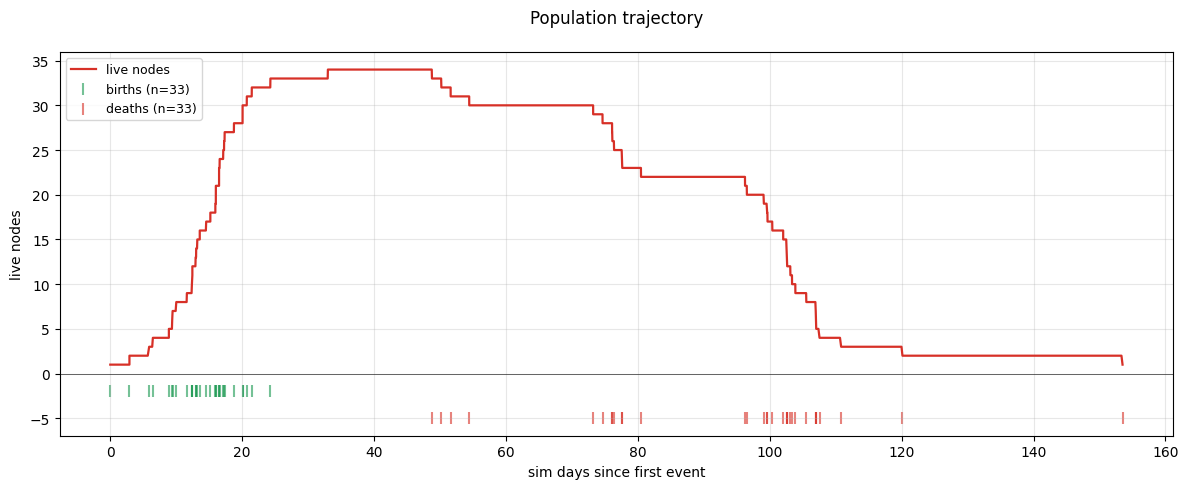
\includegraphics[width=0.6\linewidth]{figures/population_no_faucet.png}}
  \smallskip
  \small
  \begin{itemize}
    \item Every €3.27 buys exactly one day, so the fleet's
      \textbf{total lifespan is} at 3061 node-days (mean 93 days @ 33 nodes).
    \item One ``old'' survivor, as the failsafe concentrates residual funds into one node.
  \end{itemize}
  \textcolor{tud Orange}{\textbf{The closed-system prediction holds: a once-funded
  fleet cannot self-sustain.}}
\end{frame}
}


{
\setbeamerfont{itemize/enumerate body}{size=\small} % template pins lists to \normalsize
\begin{frame}{The lifespan clusters were predictable}
\smallskip
\smallskip
\smallskip
  \centerline{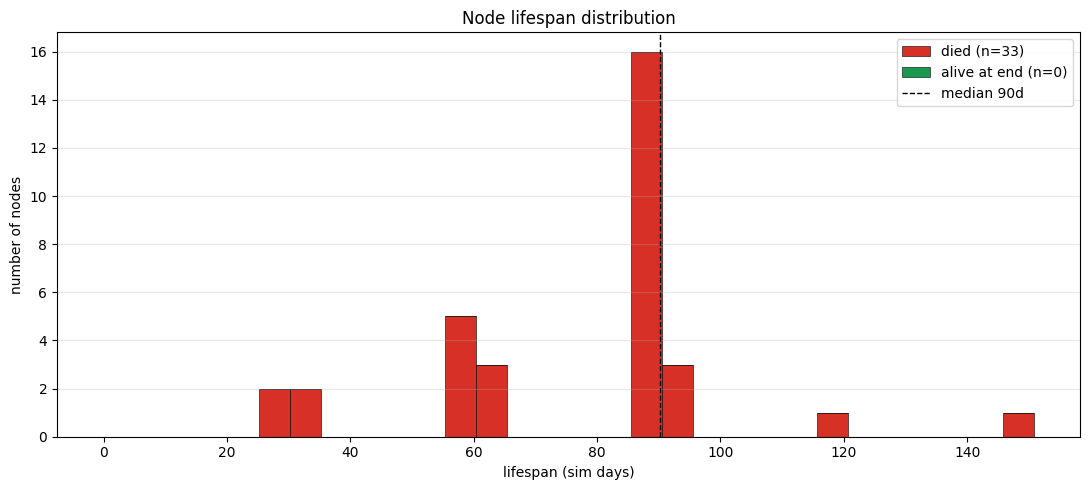
\includegraphics[width=0.65\linewidth]{figures/lifespan_hist_no_faucet.png}}

\small
Each cluster is a spawn constant: \textbf{90 d} is
      the post-spawn runway any parent retains. \textbf{60 d} and \textbf{30 d} are the last two generations of children.
  

  \begin{exampleblock}{Specification met}
    The cluster positions should be fixed, with the histogram confirming.
  \end{exampleblock}
\end{frame}
}


{
\setbeamerfont{itemize/enumerate body}{size=\small} % template pins lists to \normalsize
\begin{frame}{Income run: persistence, and an artifact}
  \framesubtitle{Open system}
  \centerline{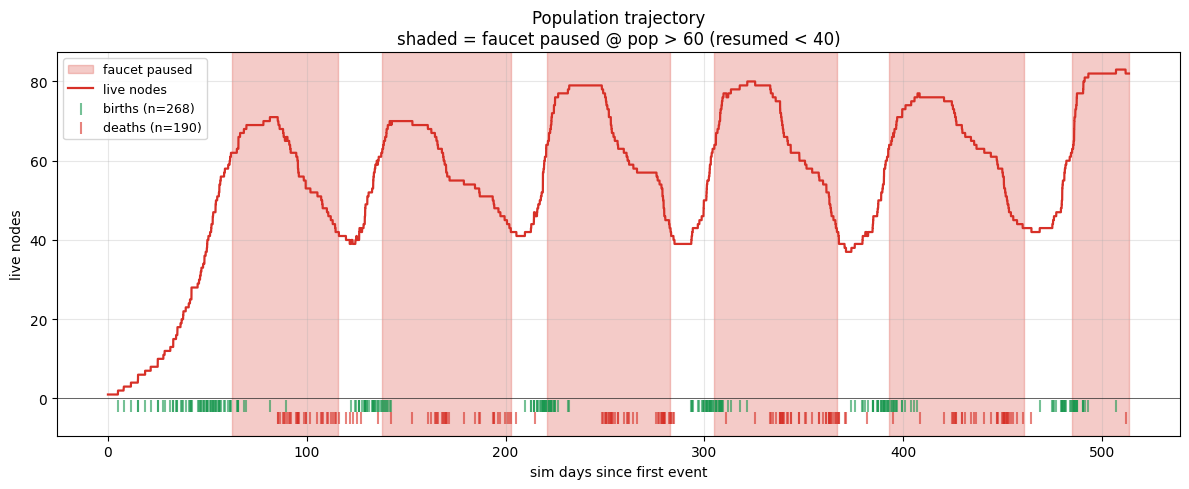
\includegraphics[width=0.54\linewidth]{figures/population_faucet.png}}
  \smallskip
  \small
  \begin{itemize}
    \item The 40--80 oscillation is an \textbf{artifact of the node cap}: the host
      tops out near 80 containers, so income is cut at 60 nodes and restored below
      40.
    \item Underneath hides a real self-limiting dynamic --- each spawn spreads
      capital over more nodes, shrinking per-node surplus --- but at these sizes the
      cap masks it (\(\to\) future work).
  \end{itemize}

  \textcolor{tud Orange}{\textbf{Income above per-node rent turns a 153-day die-off
  into persistence past 510 days.}}
\end{frame}
}


{
\setbeamerfont{itemize/enumerate body}{size=\small} % template pins lists to \normalsize
\begin{frame}{Survival without longevity}
  \framesubtitle{Lifespans, with income}
  \centerline{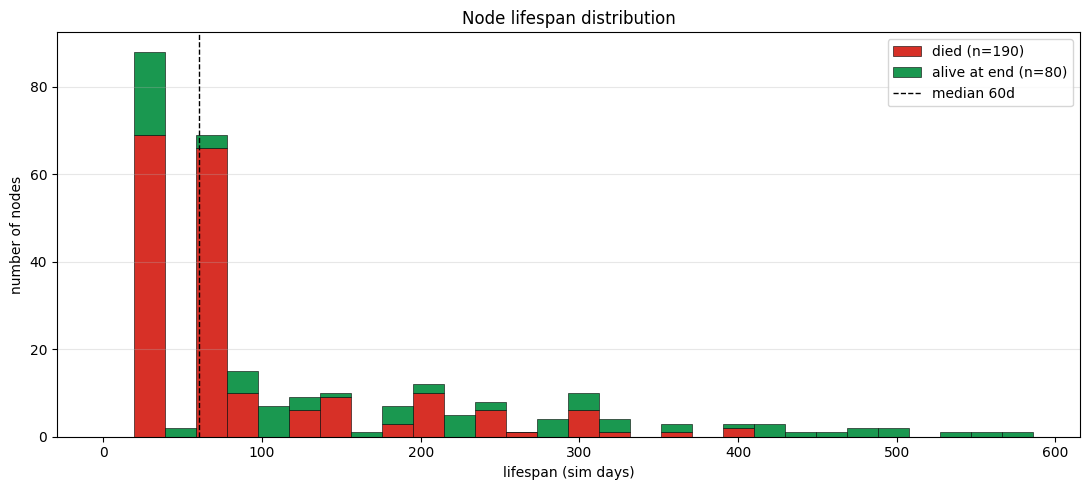
\includegraphics[width=0.42\linewidth]{figures/lifespan_hist_faucet.png}}
  \smallskip
  \small
  \begin{itemize}
    \item Uneven early income (Dirichlet shares) splits the fleet: a node drawing
      above-median income early crosses the spawn threshold with a large surplus and
      keeps 60\% of it, so \textbf{early wealth compounds} into a few long-lived
      lineages.
  \end{itemize}

  \begin{block}{The turnover principle}
    Survival needs only \emph{some} node holding a surplus, so a small well-funded
    minority replaces the short-lived majority --- the fleet tolerates high turnover
    by design.
  \end{block}
\end{frame}
}


{
\setbeamerfont{itemize/enumerate body}{size=\small} % template pins lists to \normalsize
\begin{frame}{Caution under selection: the hypothesis}
  \framesubtitle{Trait distribution of live nodes, 90-day snapshots}
  \small
  \begin{columns}[T, onlytextwidth]
    \begin{column}{0.46\textwidth}
      \centering
      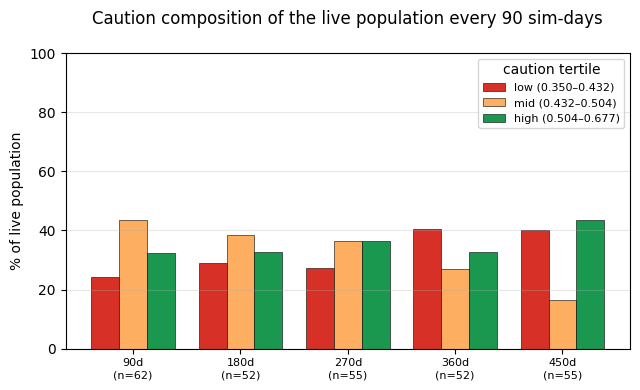
\includegraphics[width=\linewidth]{figures/caution_alive_tertiles_faucet.png}
    \end{column}
    \begin{column}{0.5\textwidth}
      Mutation is \textbf{mean-reverting toward 0.5}, yet the middle hollows while
      both extremes grow --- polarization against a centering pull means
      \textcolor{tud Orange}{genuine selection pressure} is acting.

      \smallskip
      \textbf{Hypothesis:} the income on/off cycle rewards opposite strategies ---
      low caution exploits growth (spawn aggressively), high caution survives
      drought (hoard runway), mid caution exploits neither.

      \smallskip
      Two falsifiable predictions:
      \begin{enumerate}
        \item low caution reproduces faster during income;
        \item high caution dies less during drought.
      \end{enumerate}
    \end{column}
  \end{columns}
\end{frame}
}


{
\setbeamerfont{itemize/enumerate body}{size=\small} % template pins lists to \normalsize
\begin{frame}{Caution under selection: the result}
  \framesubtitle{Birth and death rates by caution group and phase}
  \small
  \begin{columns}[T, onlytextwidth]
    \begin{column}{0.42\textwidth}
      \centering
      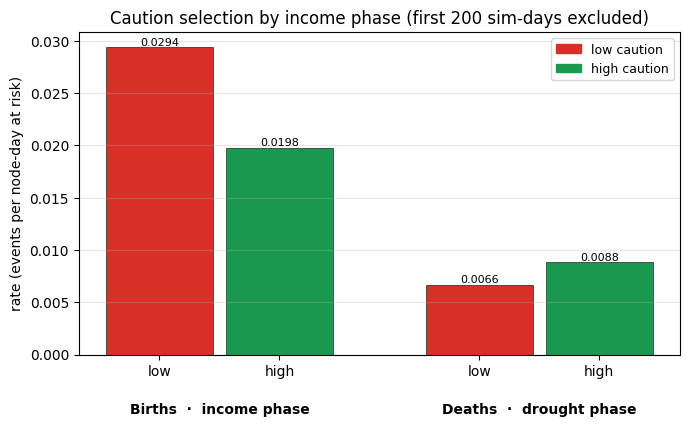
\includegraphics[width=\linewidth]{figures/caution_birth_death_diff.png}
    \end{column}
    \begin{column}{0.54\textwidth}
      \begin{exampleblock}{Prediction 1 --- confirmed}
        Low caution reproduces \(\sim\)50\% faster while income flows
        (0.0294 vs.\ 0.0198 births/day).
      \end{exampleblock}
      \begin{alertblock}{Prediction 2 --- disconfirmed}
        No survival edge --- high caution even dies slightly \emph{more} in drought
        (0.0088 vs.\ 0.0066 per day). Selection favored low caution: the reproduction
        gap ran in every phase.
      \end{alertblock}

      {\footnotesize The environment was \textbf{income-dominated} --- pauses too
      short for caution to pay off. The mechanism works; testing the survival half
      awaits sustained scarcity (\(\to\) future work).}
    \end{column}
  \end{columns}
\end{frame}
}

%
% Segment 5 --- Viability & validity (slides 17--18). Steps back from the runs
% to ask what they cost and what they prove. No new figures: slide 17 distills
% the storage-economics table to the cost comparison; slide 18 is the
% internal-vs-external validity split. Numbers verbatim from the thesis
% (conclusion.tex, limitations.tex, discussion.tex).
%

{
  \renewcommand{\sectionsubtitle}{Economics, and the limits of the evidence}
  \section{Viability \& validity}
}


{
\setbeamerfont{itemize/enumerate body}{size=\small} % template pins lists to \normalsize
\footerinfootnotestrue % full-reference footnote -> move footer into footnote band
\begin{frame}{Not cost-competitive --- and that is the point}
  \framesubtitle{Storage economics}
  \small
  \begin{columns}[T, onlytextwidth]
    \begin{column}{0.44\textwidth}
      \textbf{Cost per TB-month}

      \smallskip
      \begin{tabular}{@{}lr@{}}
        EternalSeedBox            & \textbf{€241} \\
        Commercial object storage & €20--25 \\
        \hline
        Premium                   & \(\approx 10\times\) \\
      \end{tabular}

      \smallskip
      {\footnotesize Commercial \(=\) object-storage list
      price.\cite{cloud_storage_pricing}}

      \medskip
      {\footnotesize Break-even \textbf{€3.27 / node / day}
      (€98 per 30 d, 400 GB served).}
    \end{column}
    \begin{column}{0.52\textwidth}
      \begin{block}{A deliberate niche, not a general store}
        Each node pays \textbf{retail VPS} --- no economies of scale, so the rate
        cannot match commercial storage. The premium buys availability that
        \textbf{survives takedown} and open-source accountability. The market is
        users whose content no one else will host, funding the infrastructure
        directly.
      \end{block}
    \end{column}
  \end{columns}

  \textcolor{tud Orange}{\textbf{Competitive only where availability itself is the
  product.}}
\end{frame}
}


{
\setbeamerfont{itemize/enumerate body}{size=\small} % template pins lists to \normalsize
\begin{frame}{What the runs establish --- and what they cannot}
  \framesubtitle{Threats to validity}
  \small
  \begin{columns}[T, onlytextwidth]
    \begin{column}{0.46\textwidth}
      \begin{exampleblock}{Internal validity --- strong}
        \begin{itemize}
          \item Unmodified production code against faithful \textbf{Bitcoin} and
            \textbf{VPS-marketplace} replicas.
          \item Replication verified under \textbf{both} the closed and income
            conditions.
          \item The closed-system prediction was met.
        \end{itemize}
      \end{exampleblock}
    \end{column}
    \begin{column}{0.5\textwidth}
      \begin{alertblock}{External validity --- open}
        \begin{itemize}
          \item Node cap 60 --- host ceiling (\(\sim\)60--80 containers), not
            economics.
          \item Regtest drops \(\sim\)50\% of tx \(\to\) income set \(10\times\)
            rent \(\to\) economy inflated.
          \item Single VPS provider (SporeStack) --- no failover.
          \item Revenue mechanism not yet designed.
          \item Fixed genesis catalog.
        \end{itemize}
      \end{alertblock}
    \end{column}
  \end{columns}

  \textcolor{tud Orange}{\textbf{The mechanism is validated; viability is not ---
  by construction.}}
\end{frame}
}

% \splitpos and the footer-white flag are stateful --- set inside the group and
% reset after it.

{
  \renewcommand{\sectionsubtitle}{Limitations, and what comes next}
  \section{Conclusion}
}


{
\setbeamerfont{itemize/enumerate body}{size=\small} % template pins lists to \normalsize
\setlength{\splitpos}{0.55\paperwidth} % colored pane left, title shifts right
\leftfooterwhitetrue
\begin{frame}{The answer}
  \begin{columns}[T]
    \begin{textcolumn}
      \color{white}\large
      \textbf{Yes --- conditional.}

      \medskip
      The fleet survives and grows after genesis \textbf{when its income
      covers or exceeds the per-node rent.}
    \end{textcolumn}
    \begin{textcolumn}
      \small
      \textbf{Three contributions:}
      \begin{enumerate}
        \item \textbf{Engineering} --- first self-replicating economic agent that
          buys real infrastructure on an open market.
        \item \textbf{Method} --- unmodified production code against faithful
          Bitcoin + VPS-marketplace replicas.
        \item \textbf{Empirical} --- fleet dynamics and one heritable trait under
          selection. A prediction met, one not observed.
      \end{enumerate}
    \end{textcolumn}
  \end{columns}
\end{frame}
}
\setlength{\splitpos}{0pt}\leftfooterwhitefalse % reset stateful split/footer


{
\setbeamerfont{itemize/enumerate body}{size=\small} % template pins lists to \normalsize
\setlength{\splitpos}{0.55\paperwidth} % colored pane left, title shifts right
\leftfooterwhitetrue
\begin{frame}{Future work}
  \begin{columns}[T]
    \begin{textcolumn}
      \color{white}
      {\Large\textbf{Thank you!}}

      \medskip
      {\large Questions?}
    \end{textcolumn}
    \begin{textcolumn}
      \small
      \begin{itemize}
        \item \textbf{Payment incentive} --- make consumers fund seedboxes
          directly.
        \item \textbf{Decentralized moderation} --- solve removal requests
          across a fleet with no central authority.
        \item \textbf{Longer drought, no node cap} --- to test the unconfirmed
          survival half of the caution hypothesis and better observe large-scale fleet dynamics.
      \end{itemize}
    \end{textcolumn}
  \end{columns}
\end{frame}
}
\setlength{\splitpos}{0pt}\leftfooterwhitefalse % reset stateful split/footer









\begin{frame}[allowframebreaks,t]{\bibname}
  % the 'I' is caused by 'allowframebreaks'
  \AtNextBibliography{\footnotesize}% or in the preamble \AtBeginBibliography{\small}
  \printbibliography
\end{frame}

\end{document}
